\section{Bases ortonormales de espacios de Hilbert}
\label{Bases ortonormales de espacios de Hilbert}
\TODO{ver si, junto con G-S, puedo subir esto.}

En general, dado un $F-$espacio vectorial $V$,
si uno acepta el axioma de elección, siempre cuenta con 
bases para este espacio,
es decir, de subconjuntos de $V$ que son tanto linealmente
independientes (término abreviado como ``l.i.'') como generadores
de todo el espacio; la importancia de 
estas es obvia pues, por definición, una base permite representar
de forma única a un elemento $v \in V$ por medio
de una colección de escalares. 


Puede demostrarse
que, dado $A \subseteq V$, el que $A$ sea base de $V$
equivale a que $A$ sea un maximal linealmente
independiente (c.f. sección 1.7 de \cite{friedberg}), es decir,
que todo subconjunto  linealmente
independiente de $V$ que contenga
a $A$ de hecho coincide con $A$.


El tener además en $V$ definido un producto punto
dota de estructura extra al espacio, en particular, 
como dijimos ya,
nos provee de una noción de longitud (
c.f. proposición \ref{prop: La norma inducida por un producto punto}) 
y también 
de ortogonalidad (\TODO{ref}), luego, en este 
contexto podemos también hablar de subconjuntos $B$
ortonormales maximales. Puesto que la ortogonalidad implica
trivialmente la independencia lineal, es natural plantearse
la siguiente pregunta: en un $F-$espacio vectorial $V$
con producto punto
cualquiera, ¿es cierto que todo ortonormal maximal es también
maximal l.i., o sea, una base
del espacio? 

Antes de proceder, 
conviene dejar por escrito estos dos conceptos.

\begin{defi} \label{defi: BON y base de Hamel}
Sea $V$ un espacio vectorial con producto punto.
Si $A$ es un subconjunto de $V$ que es 
maximal con respecto a la propiedad de
\begin{itemize}
\item ser linealmente independiente, entonces lo llamaremos
\textbf{base de Hamel} de $V$
\item ser ortonormal, entonces lo llamaremos
\textbf{base ortonormal} de $V$ (y abreviamos este
nombre como \textbf{BON}).
\end{itemize}
\end{defi}


Como se establece 
fácilmente en la siguiente proposición,
\textit{en el caso finito dimensional}, la respuesta a la pregunta
planteada es positiva.

\begin{prop}
\textbf{(en espacios de Hilbert de dimensión finita, toda BON es
base de Hamel)}
\label{prop: en dimension finita toda BON es base de Hamel}
Sea $V$ un espacio finito dimensional
con producto punto. Si $A$
es un subconjunto ortonormal maximal de $V$, entonces
también es maximal l.i. (o sea, base de $V$)
\end{prop}
\noindent
\textbf{Demostración.}
Supongamos que $A \subseteq V$ es maximal 
respecto a la propiedad de ser ortonormal pero
no a la de ser l.i., es decir, que existe
un subconjunto $A'$ l.i. que contiene a $A$ propiamente.
Digamos que $A' = A \cup B$.
Podemos ortonormalizar a este con el proceso de Gram-Schmidt
para obtener un subconjunto ortonormal $A´´$ de
$V$ que genera 
el mismo espacio que genera $A'$;
por las fórmulas del teorema \ref{Teo:Gram-Schmidt}
y el hecho de que los elementos de $A$ sean ortogonales
entre sí es claro que los primeros $|A|$ elementos
son los elementos de $A$ (``intactos''); así $A''$
es un subconjunto ortonormal de $V$ que contiene propiamente
a $A$ (contradicción).
\QEDB
\vspace{0.2cm}


Como se comenta en \cite{mse1},
en el caso en el que el espacio de Hilbert $V$
no sea infinito-dimensional, \textbf{una base 
Hamel de este espacio no puede ser una
base ortonormal del espacio.}

Así, en general los sistemas de representación
descritos en la definición 
\ref{defi: BON y base de Hamel} no son equivalentes.
A pesar de que
\begin{itemize}
	\item todo espacio de Hilbert tiene bases de Hamel, aunque
	no necesariamente bases ortonormales (c.f. 
	\cite{mse2}), y que
	
	\item si $\cali{B}$ es una base Hamel uno \textit{siempre}
	puede representar cualquier vector $x$ del espacio como combinación
	lineal \textit{finita} de elementos de $\cali{B}$, mientras que,
	si $\cali{B}$ es una BON, se tienen no igualdades entre 
	$x$ y combinaciones lineales de elementos de $\cali{B}$, sino aproximaciones
	del primero a partir de los segundos (c.f. inciso d)
	del teorema \ref{thm: Coway, 4.13}),
\end{itemize}

\noindent
como mostraremos más adelante, en el contexto de
espacios de Hilbert, conviene mucho más trabajar con BONs
(cuando existen para el espacio particular)
que con bases de Hamel. 


Es por eso que en la mayoría
de los libros de análisis funcional, el nombre ``base''
suele ser sinónimo de 
``base ortonormal''
(pudiendo llegar a confundir
a un lector primerizo, y llevarlo a pensar en
bases de Hamel). Puesto que
nosotros no queremos dar lugar a confusiones de este estilo,
nos abstenemos de usar el nombre ``base'' y en su lugar ocupamos
los nombres introducidos en la definición \ref{defi: BON y base de Hamel}.

\subsection{El concepto de redes como un generalización del de sucesión}

Para dar unas equivalecias útiles a la propiedad de
ser base ortonormal de un espacio de Hilbert, requeriremos del
del concepto de ``red'', usado en topología como una extensión
de la noción de sucesión.

\marginnote{Para más detalles sobre redes, consulte \cite{munkres}
p.87}

Puede recordar la definición de ``orden parcial'' en 
\cite{munkres} p. 187; el único tipo de conjunto parcialmente
ordenado (abreviado ``POSET'') que aquí nos interesa es 
aquel ordenado por la relación "$\subseteq$" (o sea, por la contención).
\begin{defi}
\label{def: conjunto dirijido}
Sea $(\cali{E}, \leq )$ un orden parcial. Si para cualesquiera
$\alpha, \beta \in \cali{E}$ existe un $\gamma \in \cali{E}$ tal que
$\alpha \leq \gamma$ y $\beta \leq \gamma$, diremos que 
$(\cali{E}, \leq)$ es un \textbf{conjunto dirigido}. 
\end{defi}

\begin{marginfigure}
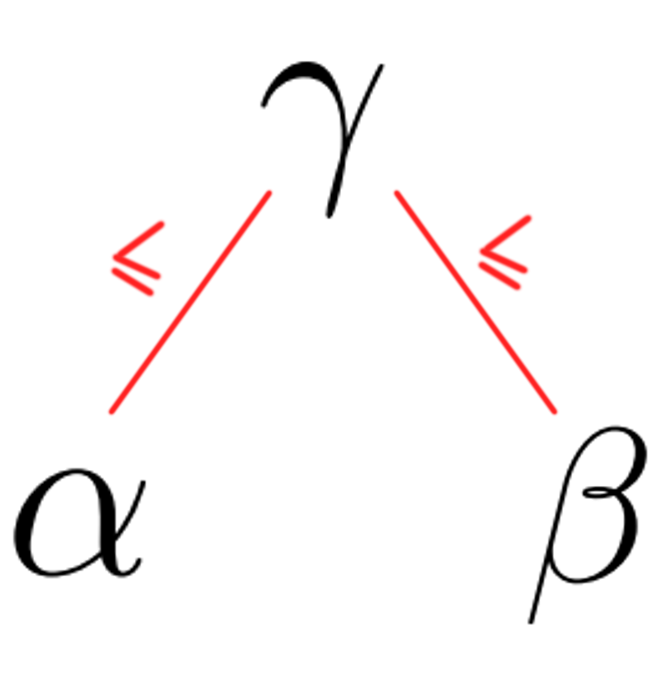
\includegraphics[scale=0.7]{net} 
		\caption{Para que un POSET $(\cali{E}, \leq)$ sea llamado ``conjunto
		dirigido'' debe cumplirse que, dados dos elementos 
		arbitrarios de $\cali{E}$ siempre sea posible encontrar un tercer
		elemento ``arriba'' de ambos.}
\end{marginfigure}


\begin{defi}
Si $(V, \tau)$ es un espacio topológico y $(\cali{E}, \leq)$ es un conjunto
dirijido, entonces a toda función $f: \cali{E} \longrightarrow V$
se le llamará una \textbf{red}.
\end{defi}

\begin{defi}
\label{def: net que converge}
Si $f: \cali{E} \longrightarrow V$ es una red, decimos que $f$ 
\textbf{converge} a un elemento del espacio $v \in V$ si 
para cualquier vecindad $U$ de $v$ (i.e. cualquier elemento
de $\tau$ que contenga a $v$) existe un $\alpha \in \cali{E}$ tal que
\[
\forall \beta \in \cali{E}: \hspace{0.2cm} 
\alpha \leq \beta \Rightarrow f(\beta) \in U.
\]
\end{defi}



Sea $(V, \langle \cdot , \cdot\rangle)$ un espacio de Hilbert;
dado un subconjunto $W = \{ v_{i} : \hspace{0.2cm} i \in I \}$
de $V$, queremos ``sumar todos los elementos de 
$W$''; puesto que trabajamos en un espacio vectorial,
la acción de sumar una cantidad \textit{finita} de elementos
de $V$ tiene sentido, pero como
\textit{a priori} no se ha supuesto nada
sobre la cardinalidad del conjunto de índices $I$, 
en general no siempre tiene sentido intentar sumar los elementos de $W$;
definimos rigurosamente esta acción a partir de una
de una red que definimos como sigue; consideramos al conjunto


\begin{comment}
{
\Huge{$\alpha$}

\Huge{$\beta$}\\

\Huge{$\gamma$}
}
\end{comment}

\begin{equation}
\label{eq0: 14ap}
\cali{P} := \{ \alpha \subseteq I : \hspace{0.2cm} \alpha \hspace{0.1cm} \textit{es finito} \}.
\end{equation}

\noindent 
Observe que $\cali{P}$ consta exactamente de los subconjuntos $\alpha$
de $I$ para los que la expresión 
\[
\suma{i \in \cali{P}}{}{v_{i}}
\]
tiene sentido. Teniendo ya un espacio topológico $(V, \tau)$
(con la topología $\tau$ definida como en
\eqref{eq: top espacio con producto punto})
y el conjuto dirigido $(\cali{P}, \subseteq)$,
definimos la siguiente red;

\begin{center}
\label{eq: net a partir de un subconjunto de un espacio de Hilbert}
$\aplica{f_{\cali{P}}}{\cali{P}}{V}{\alpha}{ \suma{i \in \alpha}{}{v_{i}.}}$
\end{center}

El que esta red converja (c.f. definición
\ref{def: net que converge}) a un $v \in V$ significa que
para todo $\epsilon >0$ exista $\alpha \subseteq I$
finito tal que, si $\beta$ es otro subconjunto finito de $I$
que contenga a $\alpha$, entonces
\[
\left| \suma{i \in \beta}{}{v_{i}} - v \right| < \epsilon;
\]

\noindent o sea, que $\suma{i \in \alpha}{}{v_{i}}$
se encuentra a distancia $\epsilon$ de $v$ y que, no importa
cuántos sumandos se agregen, la suma resultante sigue siendo 
un vector que se encuentra a 
distancia $\epsilon$ de $v$.

\begin{notacion}
Si la red $f_{\cali{P}}$ converge,
denotaremos a su límite como
$\suma{}{}{\{ v_{i}: \hspace{0.2cm} i \in I \}}$.
\end{notacion}

\begin{nota}
Si el conjunto de índices $I$ es infinito numerable, ya 
teníamos una forma natural de definir la suma 
de los elementos de $W = \{ v_{i}: \hspace{0.2cm} i \in I \}$;
haciendo $I = \IN$ (mejor dicho, identificando a $I$ con 
$\IN$ via una biyección), podiamos preguntarnos por la existencia
del límite de la sucesión de sumas parciales
$\suma{i=1}{n}{v_{i}}$; \textbf{debe tener cuidado}, pues
la convergencia de la \textbf{red} $f_{\cali{P}}$ definida como 
$f_{\cali{P}}(\alpha) = \suma{i \in \alpha}{}{v_{i}}$ 
(con $\alpha \subseteq \IN$ cualquier subconjunto finito de $\IN$)
\textbf{no}
equivale a la convergencia de la \textbf{sucesión}
$\left( \suma{i=1}{n}{v_{i}} \right)_{n \in \IN}$
(c.f. p. 16 de \cite{conway}). \\
De existir, al límite de la red lo denotamos por
$\suma{}{}{\{ v_{i} : \hspace{0.2cm} i \in \IN \}}$, mientras
que al límite de la sucesión lo denotamos por
$\suma{i=1}{\infty}{v_{i}}$.
\end{nota} 


\subsection{Caracterización y propiedades de las bases ortonormales de un espacio de Hilbert}


Enunciamos y demostramos el teorema
\ref{thm: Coway, 4.13}, en el que damos algunas equivalencias
a ser base ortonormal.

Para la demostración necesitamos antes del siguiente lema,
cuya demostración puede consultarse en \cite{conway}, p. 16.

\begin{lema}
\label{lema: 4.12 conway}
\textbf{(Lema 4.12 de \cite{conway})}
Sean $(V, \langle \cdot , \cdot \rangle)$ un espacio
de Hilbert, $\cali{E}= \{e_{i}: \hspace{0.2cm} i \in I \}$ 
un subconjunto ortonormal de
$V$. Si $x \in V$ es un elemento arbitrario del espacio,
$W := \{ \langle x, e_{i} \rangle:\hspace{0.2cm} i \in I \}$
y $\cali{P}:= \{ \alpha \subseteq I: \hspace{0.2cm} \alpha \text{ finito} \}$,
entonces la red
$f_{\cali{P}}: \cali{P} \longrightarrow V$ 
definida como $f(\alpha) = \suma{i \in \alpha}{}{\langle x, e_{i} \rangle e_{i}}$
converge a un elemento de $V$ que denotamos por 
$\suma{}{}{ \{ \langle x, e \rangle e: \hspace{0.2cm} e \in \cali{E} \} }$.
\end{lema}



\begin{teo} \label{thm: Coway, 4.13}
\textbf{(Teorema 4.13 de \cite{conway} )}
Sea $\cali{E}$ un subconjunto ortonormal del espacio
de Hilbert $(V, \langle \cdot , \cdot \rangle)$.
Las siguiente proposiciones son equivalentes entre sí:
\begin{itemize}
\item[a)] $\cali{E}$ es una BON de $V$ (en el sentido
de la definición \ref{defi: BON y base de Hamel}).
\item[b)] Si $x \in V$ es ortogonal a todo elemento de 
$\cali{E}$ entonces $x=0$.
\item[c)] $\overline{span}(\cali{E})= V$.
\item[d)] Para todo $x \in V$ se cumple que
\[
x = \suma{}{}{\{ \langle x,e \rangle e | e \in \cali{E} \}}
\]
\item[e)] Para cualesquiera $x, y \in V$,
\[
\langle x,y \rangle= \suma{}{}{\{ \langle x,e \rangle  \langle e,y \rangle | e \in \cali{E} \}}
\]
\item[f)](\textbf{Identidad de Parseval})
Para todo $x \in V$ se cumple que
\[
||x||^{2}= \suma{}{}{\{ \langle x,e \rangle ^{2} | e \in \cali{E} \}}.
\]
\end{itemize}
\end{teo}

\marginnote{
El inciso $c)$ del teorema 
\ref{thm: Coway, 4.13}
corresponde a la definición
de BON dada en \cite{kolmogorov}; así, una BON
es también un subconjunto ortonormal tal que el menor
subespacio cerrado de $V$ que contiene a $\cali{E}$ es 
todo $V$. Compare este inciso con el hecho de que
$\cali{E}$ es una base de Hamel de $V$ si y sólo si $E$ es
linealmente independiente y $span(\cali{E}) = V$.}
\noindent
\textbf{Demostración.}
\begin{itemize}

\item[$a) \Rightarrow b)$] Suponer la existencia de un 
$x$ no cero ortogonal a todo elemento de $\cali{E}$
nos permite considerar al subconjunto ortonormal
\[
\cali{E} \cup \left\{ \frac{x}{||x||} \right\}
\]
de $V$
que contiene propiamente a $\cali{E}$,
contradiciendo así la maximalidad de $\cali{E}$
respecto a la propiedad de ser ortonormal.

\item[$b) \Rightarrow c)$] Sea el subespacio
$W := \overline{span}(\cali{E})$ de $V$. Por ser
$W$ un subespacio cerrado de $V$, podemos proyectar
sobre él (c.f. teorema \ref{Teo:proyOrt}).
Para mostrar que tenemos la igualdad entre
$V$ y $W$, tomemos un $x \in V$ cualquiera.
Según el teorema de la proyección ortogonal 
\ref{Teo:proyOrt}, $x-\Pi_{W}(x)$
es ortogonal a todo elemento de $W$, 
en particular, será ortogonal a todo elemento de
$\cali{E}$ (pues $\cali{E} \subseteq W$);
por hipótesis, esto implica que $x-\Pi_{W}(x)$ sea el vector cero;
así,
\[
x = \Pi_{W}(x) \in W.
\]

\item[$c) \Rightarrow b)$] Sea $v \in V$
ortogonal a todo elemento de $\cali{E}$; mostremos que
$v$ es cero. Como $v \in V = \overline{span}(\cali{E})$,
existe $(b_{n})_{n \in \IN}$ una sucesión de
$span(\cali{E})$ tal que
$\lim_{n \rightarrow \infty}b_{n}=v$ 
(c.f. lema 21.2 de \cite{munkres}).
Usando el que para toda $n$ el producto punto 
$\langle b_{n}, h \rangle$
sea cero y la continuidad
establecida en la proposición \ref{prop: continuidad del producto punto},
llegamos a que
\[
\langle x,x \rangle= \langle x, \lim_{n \rightarrow \infty}b_{n} \rangle= 
\lim_{n \rightarrow \infty} \langle x, b_{n} \rangle= 
\lim_{n \rightarrow \infty} 0 = 0,
\]
de donde concluimos 
(c.f. \eqref{eq: norma via producto punto} y 
definición \ref{def: prod punto})
que $x$ es cero.
 

\item[$b) \Rightarrow d)$] Según el lema \ref{lema: 4.12 conway},
la red $f_{\cali{E}}$ converge a un vector, que denotamos por 
$\suma{}{}{\{ \langle x,e \rangle e | e \in \cali{E} \}}$;
resta ver que tal 
vector es $x$
o, equivalentemente, que
$
\suma{}{}{\{ \langle x,e \rangle e | e \in \cali{E} \}} -x
$
es el vector cero; según nuestra hipótesis, podremos
concluir esto si demostramos que para todo $e \in \cali{E}$
ocurre

\begin{equation}
\label{eq2: 14ap}
\langle \suma{}{}{\{ \langle x,e \rangle e | e \in \cali{E} \}} -x, e \rangle
= 0.
\end{equation}

Fijempos pues un $e \in \cali{E}$ y sea
$\epsilon >0$.
Por definición de convergencia de redes, sabemos que
existe $F \subseteq \cali{E}$ finito con $e \in F$
tal que
\begin{equation} \label{eq 1: 8Agosto}
|L_{F}| < \epsilon,
\end{equation}
donde $L_{F}:= \suma{f \in F}{}{ \langle x,f \rangle f } - 
\suma{}{}{\{ \langle x,e \rangle e| e \in \cali{E} \}} \in V$, o sea,

\begin{equation}
\label{eq1: 14ap}
\suma{}{}{\{ \langle x,e \rangle e| e \in \cali{E} \}}
= \suma{f \in F}{}{ \langle x,f \rangle f } - L_{F}
\end{equation}

Por la bilinealidad del producto punto y por
ser $e$ ortogonal a todo elemento de $\cali{E}-\{ e \}$
tenemos que
\begin{equation} \label{eq 2: 8Agosto}
\langle \suma{f \in F}{}{\langle x,f \rangle f}, e \rangle = \suma{f \in F}{}{
\langle x,f \rangle \langle f,e \rangle}
= \langle x,e \rangle \langle e,e \rangle =
\langle x,e \rangle.
\end{equation}

Así,
\begin{align*}
0 \leq & | \langle \suma{}{}{\{ \langle x,e \rangle e | e \in \cali{E} \}} -x, e \rangle | \\
= &
| \langle \suma{}{}{\{ \langle x,e \rangle e | e \in \cali{E} \}}, e \rangle - 
\langle x, e \rangle| \\
(\text{por } \eqref{eq1: 14ap}) = & 
| \langle 
\suma{f \in F}{}{ \langle x,f \rangle f  } - L_{F}, e
\rangle - 
\langle x, e \rangle | \\ 
= & 
| \langle 
\suma{f \in F}{}{ \langle x,f \rangle f  }, e \rangle  
- \langle L_{F}, e \rangle - \langle x, e \rangle | \\
(\text{por \eqref{eq 2: 8Agosto} }) = & 
|
\langle x, e \rangle
- \langle L_{F}, e \rangle - \langle x, e \rangle |  \\
= & | \langle L_{F}, e \rangle | \\
(\text{Cauchy-Schwarz}) \leq & ||L_{F}|| \cdot ||e|| = |L_{F} | \\
(\text{por \eqref{eq 1: 8Agosto}}) \leq  &  \epsilon;
\end{align*}

\noindent
demostramos así que
\[
\forall \epsilon > 0: \hspace{0.2cm} 
0 \leq  | \langle \suma{}{}{\{ \langle x,e \rangle e | e \in \cali{E} \}} -x, e \rangle | \leq  \epsilon;
\]
de esto concluimos que $ | \langle \suma{}{}{\{ \langle x,e \rangle e | e \in \cali{E} \}} -x, e \rangle |$ es cero, de donde se deduce, como queríamos, \eqref{eq2: 14ap}.


\item[$d) \Rightarrow e)$] Según nuestra hipótesis,
\[
x= \suma{}{}{\{ \langle x,e \rangle e | e \in \cali{E} \}}, \hspace{0.5cm}
y= \suma{}{}{\{ \langle y,e \rangle e | e \in \cali{E} \}}.
\]

\noindent
Para $F \subseteq \cali{E}$ finito, sean
\[
X_{F}:= \suma{e \in F}{}{\langle x, e \rangle} e -x,
\hspace{0.5cm}
Y_{F}:= \suma{e \in F}{}{\langle y, e \rangle} e -y.
\]

Por la ortonormalidad supuesta en el conjunto $\cali{E}$,
\begin{equation}
\label{eq 3: 8Agosto}
\left\langle \suma{e \in F}{}{\langle x, e \rangle e}, 
\suma{e \in F}{}{\langle y, e\rangle e} \right\rangle
= \suma{e \in F}{}{
\langle  x,e \rangle \langle y,e \rangle};
\end{equation}
así,



\begin{align*}
|\suma{e \in F}{}{\langle x,e \rangle \langle y,e \rangle } - 
\langle  x,y \rangle | & \underbrace{=}_{\text{por 
\eqref{eq 3: 8Agosto}}} |\left\langle \suma{e \in F}{}{\langle x, e\rangle e}, \suma{e \in F}{}{\langle y, e\rangle e} \right\rangle
- \langle x,y\rangle | \\
= & |\langle X_{F}+x, Y_{F}+y \rangle  - \langle x,y\rangle | \\
= & |\langle X_{F}, Y_{F}\rangle + \langle X_{F}, y\rangle  + 
\langle x,Y_{h}\rangle | \\
(\text{desigualdad triangular}) \leq & |\langle X_{F}, Y_{F}\rangle  | + 
|\langle X_{F}, y \rangle |
+ |\langle x,Y_{H}\rangle | \\
(\text{Cauchy-Schwarz}) \leq & ||X_{F}|| \cdot ||Y_{F}|| +
||X_{F}|| \cdot ||y|| + ||x|| \cdot ||Y_{H}||;
\end{align*}
puesto que $||x||$ y $||y||$ son constantes
y $||X_{F}||$ y $||Y_{F}||$ pueden hacerse tan pequeñas como
se quiera (escogiendo apropiadamente al conjunto finito $F$),
concluimos que
$\suma{}{}{ \{ \langle x,e \rangle \langle y, e \rangle: \hspace{0.2cm} e \in \cali{E} \}}
= \langle x, y \rangle$.

\item[$e) \Rightarrow f)$] Para $x \in V$,
\[
||x||^{2}=\langle x,x \rangle = \suma{}{}{\{
\langle x,e\rangle ^{2}| e \in \cali{E} \}}.
\]

\item[$f) \Rightarrow a)$]
Supongamos que $\cali{E}$ puede extenderse aún más
para ser ortonormal, es decir, que existe 
$e_{0} \in V$ unitario tal que
para todo $e \in \cali{E}$ se tenga que 
$\langle e_{0}, e \rangle=0$. 
Llegamos entonces a la siguiente contradicción:
\[
1=||e_{0}||^{2}=\suma{}{}{\{ 
\langle e_{0}, e \rangle^{2}| e \in \cali{E} \}}=
\suma{}{}{\{ 0\}}=0.
\]
\QEDB
\end{itemize}
\vspace{0.2cm}


\begin{nota}
\label{nota: sobre la identidad de parseval}
\textbf{(sobre la identidad de Parseval en el
caso finito dimensional)}
Puesto que, para el desarrollo teórico de este trabajo de tesis,
se tratará siempre con espacios de Hilbert finito dimensionales, luego, con
bases ortonormales finitas, conviene
reescribir algunos puntos del teorema 
\ref{thm: Coway, 4.13} en este caso particular.
Digamos que $dim(V)=n$; si 
$\cali{E} := \{e_{k}: \hspace{0.2cm} 0 \leq k \leq n-1 \}$ es una
BON del espacio de Hilbert $V$, entonces, para todo
$x \in V$, se tiene que 

\begin{equation}
\label{eq0: 11ap}
x = \suma{k=0}{n-1}{\langle x , e_{k} \rangle^{2} e_{k}}
\end{equation}
y además

\begin{equation}
\label{eq1: 11ap}
|| x ||^{2} = \suma{k=0}{n-1}{\langle x , e_{k} \rangle^{2}};
\hspace{0.4cm} \textit{(Identidad de Parseval)}
\end{equation}


\noindent
así, si se usa a una BON $\cali{E}$ del espacio como sistema
de representación (o sea, si se representa a todo $x$ del espacio 
por medio de sus $n$ coeficientes respecto a $\cali{E}$), se tiene que
\begin{itemize}
	\item tales coeficientes son de hecho los productos punto entre
	$x$ y los elementos de la base $\cali{E}$ (c.f. 
	\eqref{eq0: 11ap}), y
	\item se tiene una relación lineal muy sencilla entre el cuadrado
	de la norma de $x$ y el cuadrado de los coeficientes de la representación
	(c.f. \eqref{eq0: 11ap}).
\end{itemize}

Estos dos hechos permiten \textbf{usar la magnitud de un coeficiente en 
\eqref{eq0: 11ap} para valorar la contribución del respectivo 
elemento de la base $\cali{B}$ para sintetizar a $x$};
en efecto, si, por ejemplo, el coeficiente $\langle x, e_{k_{1}} \rangle$
es ``muy cercano a cero'', digamos $\langle x, e_{k_{1}} \rangle = \epsilon$,  
entonces el vector 
$x_{k_{1}}:= \suma{\substack{ {k=0}, \\  {k \neq k_{1}} }}{n-1}{
\langle x , e_{k} \rangle^{2} e_{k}}$
es, en la misma medida, cercano al vector inicial $x$, pues
\[
|| x - x_{k_{1}} || = || \langle x , e_{k_{1}} \rangle^{2} e_{k_{1}} ||
= \langle x , e_{k_{1}} \rangle^{2} = \epsilon.
\]
\end{nota}


\begin{comment}
Ya estamos listos par dar un ejemplo de una BON que
no es una base de Hamel.

\begin{ejemplo}
(de un subconjunto de un espacio
con producto punto que sea maximal ortonormal pero no maximal l.i.)
\TODO{Dónde introduzco al espacio de sucesiones $\ell^{2}$??
Yo creo que justo después de G-S, o sea, justo antes de esta.}

Considere al espacio de Hilbert
\[
\ell^{2}= \{ x: \IN \longrightarrow \IR | \hspace{0.2cm} 
\suma{k=1}{\infty}{|x_{k}|^{2}}< \infty \}
\]

con el producto punto
\[
<x,y>= \suma{k=1}{\infty}{x_{k}y_{k}}.
\]

Sea el subconjunto de este
\[
\cali{B}:= \{e_{i}: \IN \longrightarrow \IR| \hspace{0.2cm} i \in \IN \},
\]

donde $e_{i}$ es la sucesión dada por la regla
\[
e_{i}(j)=\delta_{i,j}, \hspace{0.4cm} j \in \IN.
\]


\begin{itemize}
\item[i)]($\cali{B}$ es un subconjunto maximal ortonormal) 
Claro que todos los elementos de $\cali{B}$ tienen norma uno;
además, si $x \in \ell^{2}$ es tal que para todo índice $i$
se tiene la igualdad
\[
x_{i}= \suma{k=1}{\infty}{x(k)e_{i}(k)}=<x,e_{i}>=0,
\]
entonces $x$ es la sucesión cero, o sea,
el elemento cero del espacio
$\ell^{2}$. Según la equivalencia
$a) \iff b)$ del teorema \ref{thm: Coway, 4.13}, esto basta
para demostrar que $\cali{B}$ es BON de $\ell^{2}$.

\item

\end{itemize}


\TODO{AAAAA}

\end{ejemplo}
\end{comment}


Esta última nota da fuertes razones sobre la utilidad
de las bases ortonormales como sistema de representación
en espacios de Hilbert. Veamos ahora cómo
las BON también son útiles para expresar proyecciones
de un vector sobre subespacios cerrados en términos del
vector y la base ortonormal. 

Para la tarea necesitamos el siguiente resultado.


\begin{prop} \label{teo: Kol 6, p.149}
(\cite{kolmogorov}, thm. 6 p. 149)
Si $\{ e_{k} |k \in \IN \}$ es un sistema
ortonormal de un espacio de Hilbert $V$ 
y $x \in V$, entonces la expresión
\[
|| x - \suma{k=1}{\infty}{a_{k}e_{k}}  ||
\]
alcanza su mínimo para la elección de coeficientes
$a_{k}= <x , e_{k} > $.
\end{prop}

\noindent
\textbf{Nota:}
En esta proposición consideramos la situación de un subespacio
con BON numerable, pero en la demostración del resultado ya
se incluye el caso de una BON finita.

\noindent
\textbf{Demostración.}
Si $(a_{k})_{k \in \IN}$ es una sucesión de coeficientes,
como es costumbre,
en caso de existir el límite de sumas parciales
$S_{n}:= \suma{k=1}{n}{a_{k}e_{k}}$, este es un vector que denotamos
por $\suma{k=1}{\infty}{a_{k}e_{k}}$. Además,
por la continuidad de la norma,
\[
||x - \suma{k=1}{\infty}{a_{k}e_{k}} || = \limite{n \rightarrow \infty }{||x-S_{n}||}
\]
por lo que, si encontramos una elección de coeficientes $(a_{k})_{k \in \IN}$
que haga que
la sucesión $(S_{n})_{n \in \IN}$ converja y tal que las normas
$||x-S_{n}||$ (o, equivalentemente, los números $||x-S_{n}||^{2}$)
sean míminas, esa será la elección buscada. \\
Observe que, para toda $n$,
\begin{align*}
||x-S_{n}||^{2} & = <x-S_{n} , x-S_{n} > \\
\text{(bilinealidad)} & =  <x, x > - 2 < x, x_{n} > + <S_{n} , S_{n}  > \\
\text{(ortonormalidad)} & =  ||x||^{2} - 2 < x ,\suma{k=1}{n}{a_{k}e_{k}} > + 
\suma{k=1}{n}{a_{k}^{2}} \\
= & ||x||^{2} - 2\suma{k=1}{n}{a_{k}c_{k}}  + 
\suma{k=1}{n}{a_{k}^{2}},
\end{align*}
donde $c_{k}:= < x , e_{k} >$. Así,
\[
||x-S_{n}||^{2} = ||x||^{2} - \suma{k=1}{n}{c_{k}^{2}}  + 
\suma{k=1}{n}{(a_{k}-c_{k})^{2}};
\]
claro que la sucesión de coeficientes que minimiza
esta expresión es $(c_{k})_{k \in \IN}$; además, no es difícil ver
que esta candidata hace que la sucesión $(S_{n})_{n \in \IN}$
de sumas parciales converja, pues tenemos la siguiente acotación
válida para toda $n$:

\begin{equation} \label{ecuacion teor kolmogorov}
\suma{k=1}{n}{c_{k}^{2}} \leq ||x||^{2}-||x-S_{n}||^{2} \leq 
\underbrace{||x||^{2}}_{cte}.
\end{equation}

\QEDB
\vspace{0.2cm}


\begin{cor} \label{cor: proyeccion en terminos de una BON}
\textbf{(Dando explícitamente a la proyección de un vector
a un subespacio cerrado respecto a una BON de este último)}
Con la notación 
e hipótesis
de la proposición \ref{teo: Kol 6, p.149},
para todo $x \in V$
tenemos que
\[
\Pi_{W}(x) = \suma{k=1}{\infty}{<x, e_{k}>e_{k}},
\]
donde $W := \overline{\{e_{k}| k \in \IN \}}$. 
\end{cor}

\begin{cor}
\label{cor: proyeccion en terminos de BON}
\textbf{(Caso particular de \ref{cor: proyeccion en terminos de una BON} para
espacios de dimensión finita)}
Sean $V$ un espacio de Hilbert, $W$ un subespacio cerrado de $V$
y de dimensión finita. Si 
$\cali{B} = \{ e_{k}: \hspace{0.2cm} 0 \leq k \leq n \}$
es una BON de $W$, entonces, para todo $x \in V$,
\[
\Pi_{W}(x) = \suma{k=0}{n-1}{ \langle x, e_{k} \rangle e_{k}}.
\]  
\end{cor}


\begin{cor} \label{cor: representacion de un vector respecto a una BON}
Si $V$ es un espacio con producto punto 
y $B=(e_{k})_{k \in \Delta}$ es una BON de este
a lo más numerable, entonces, para todo
$x \in V$, $x = \suma{k \in \Delta}{}{<x, e_{k}>e_{k}}$
\end{cor}
\noindent
\textbf{Demostración.}
La proyección de un $x \in V$ sobre $V$ es trivialmente $x$
($x$ es el elemento de $V$ más cercano a sí mismo); según el corolario
\ref{cor: proyeccion en terminos de una BON}, esta
proyección es la serie propuesta. \QEDB
\vspace{0.2cm}

Note que, en el caso en el que $\Delta$ sea infinito numerable,
el orden en que se tome la serie de arriba no importa. Esto es porque,
independientemente del orden que se elija, siempre se tratará con
una BON del espacio. \\

\begin{cor}(\textbf{Desigualdad de Bessel})
Si $\{ e_{k} | k \in \IN \}$ es un sistema ortonormal en 
el espacio con producto punto $V$, entonces, para todo $x \in V$,
\[
\suma{k=1}{\infty}{<x , e_{k} >^{2}} \leq ||x||^{2}.
\]
\end{cor}
\noindent
\textbf{Demostración.}
Esto es una consecuencia inmediata de la acotación
\eqref{ecuacion teor kolmogorov} establecida en la demostración
del teorema \ref{teo: Kol 6, p.149}.
\QEDB
\vspace{0.2cm}



